\documentclass{article}
\usepackage{basis}
\usepackage{mathe}

\usepackage{pgfplots}
\usepackage{tikz}
\pgfplotsset{compat=1.18}
\usetikzlibrary{matrix}

%Einrückung der ersten Zeile eins Absatzes unterdrücken
\setlength{\parindent}{0pt}
% Fügt Abstand zwischen Absätzen hinzu
\setlength{\parskip}{1em}


% Papierformat und Seitenabstände
\usepackage{geometry}
\geometry{a4paper, left=3cm, right=3cm, top=2cm, bottom=4cm}


\begin{document}



\section*{Jordan'sche Normalform}

Eine Aufgabe aus den Studientagen zu \texttt{Lineare Algebra (61112)} im Wintersemester 2025/26, die mit Mitteln und Kenntnissen des Kurstextes gelöst wurde.

\subsection*{Aufgabenstellung}
Gegeben ist die Matrix
\[
C = \mat{-5&1&1&1\\-3&0&-1&-1\\0&0&1&0\\-6&1&1&2}\in\mathrm M_{44}(\R).
\]
Gesucht ist eine zu $C$ ähnliche Matrix in Jordan'scher Normalform.

\subsection*{Lösung}
\paragraph{Schritt 1} Charakteristisches Polynom, Eigenwerte und algebraische Vielfachheiten.
\begin{align*}
\chi_C = \det(XI_4 - C) = \det\mat{X+5&-1&-1&-1\\3&X&-1&0\\0&0&X-1&0\\6&-1&-1&X-2}
\end{align*}
Entwicklung über dritte Zeile.
\begin{align*}
\chi_C &= 1\cdot(X-1)\cdot\det\mat{X+5&-1&-1\\3&X&1\\6&-1&X-2}\\
&= (X-1)((X+5)(X)(X-2) + (-6) + 3 - (-6)X - (-1)(X+5)-(-3)(X-2))\\
&= (X-1)(X^3 -2X^2+5X^2-10X -3+6X+X+5+3X-6)\\
&= (X-1)(X^3+3X^2-4) = (X-1)^2(X^2+4X+4) = (X-1)^2(X+2)^2\\
\lambda_1 &= 1, \qquad \quad \alpha(\lambda_1) = 2\\
\lambda_2 &= -2, \qquad \:\alpha(\lambda_2) = 2
\end{align*}
Das charakteristische Polynom ist in Linearfaktoren zerlegbar, also gibt es eine zu $C$ ähnliche Matrix in jordan'scher Normalform.

\paragraph{Schritt 2} Bestimmung der Haupträume und Angabe der Jordanblöcke.
\begin{align*}
\eig(1) &= \Ker(C - 1\cdot I_4) = \Ker\mat{-6&1&1&1\\-3&-1&-1&-1\\0&0&0&0\\-6&1&1&1} = \Ker\mat{-6&1&1&1\\0&-3&-3&-3\\0&0&0&0\\0&0&0&0}\\
&= \Ker\mat{-6&0&0&0\\0&-3&-3&-3\\0&0&0&0\\0&0&0&0} = \Ker\mat{1&0&0&0\\0&1&1&1\\0&0&0&0\\0&0&0&0} = \lin{\mat{0\\1\\-1\\0},\mat{0\\1\\0\\-1}} = V_1^{(1)}\\
\dim V_1^{(1)} &= 2 = \alpha(\lambda_1), \qquad H_C(1) = V_1^{(1)}\\
p^{(1)} &= (2 -0) = (2), \qquad q^{(1)} = (1,1)
\end{align*}
Der erste Jordanblock ist somit $J(\lambda_1,(q^{(1)})) = J(1,(1,1))$.

\begin{align*}
\eig(-2) &= \Ker(C + 2\cdot I_4) = \Ker\mat{-3&1&1&1\\-3&2&-1&-1\\0&0&3&0\\-6&1&1&4} = \Ker\mat{-3&1&1&1\\0&1&-2&-2\\0&0&3&0\\0&-1&-1&2}\\
&= \Ker\mat{-3&0&3&3\\0&1&-2&-2\\0&0&3&0\\0&0&-3&0} = \Ker\mat{-3&0&0&3\\0&1&0&-2\\0&0&3&0\\0&0&0&0} = \Ker\mat{-1&0&0&1\\0&-1&0&2\\0&0&-1&0\\0&0&0&0}\\
&= \lin{\mat{1\\2\\0\\1}} = V_1^{(2)}\\
&\dim V_1^{(2)} \neq 2,\; \text{deshalb weiter mit }\eig^2(-2)\\
\eig^2(-2) &= \Ker(C+2\cdot I_4)^2 = \mat{0&0&0&0\\9&0&-9&-9\\0&0&9&0\\-9&0&0&9} = \Ker\mat{1&0&-1&-1\\-1&0&0&1\\0&0&1&0\\0&0&0&0}\\
&= \Ker\mat{1&0&-1&-1\\0&0&-1&0\\0&0&1&0\\0&0&0&0} = \Ker\mat{1&0&0&-1\\0&0&0&0\\0&0&1&0\\0&0&0&0} = \lin{\mat{0\\-1\\0\\0},\mat{-1\\0\\0\\-1}} = V_2^{(2)}\\
\dim V_2^{(2)} &= 2 = \alpha(\lambda_2),\qquad H_C(-2) = V_2^{(2)}\\
p^{(2)} &= (2-1, 1-0) = (1,1)\qquad q^{(2)} = (2)
\end{align*}
Der zweite Jordanblock ist somit $J(\lambda_2,(q^{(2)})) = J(-2,(2))$.

\subsection*{Angabe der Matrix in Jordan'scher Normalform}
Die folgende Matrix $J$ ist in jordan'scher Normalform und ähnlich zu $C$, d.h. es gibt eine invertierbare Matrix $S\in \mathrm M_{44}(\R)$, so dass $S^{-1}CS = J$ gilt.
\begin{align*}
J = \diag(J(1,(1,1)), J(-2,(2))) = \mat{{\color{MediumVioletRed}1}&{\color{MediumVioletRed}0}&0&0\\{\color{MediumVioletRed}0}&{\color{MediumVioletRed}1}&0&0\\0&0&{\color{Green}-2}&{\color{Green}1}\\0&0&{\color{Green}0}&{\color{Green}-2}}
\end{align*}


\newpage
\subsection*{Kontrolle}
\paragraph{Die Matrix $S$} Da $q^{(1)} = (1,1)$, können die Vektoren direkt aus $V_1^{(1)}$ übernommen werden:

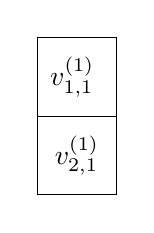
\begin{tikzpicture}[
  square/.style={
    draw,
    minimum width=1cm,
    minimum height=1cm,
    align=center
  }
]
\centering
\matrix[matrix of nodes,
        nodes={square},
        row sep=-\pgflinewidth,
        column sep=-\pgflinewidth] (grid) {
  $v_{1,1}^{(1)}$ \\
  $v_{2,1}^{(1)}$\\
};
\end{tikzpicture}

\[v_{1,1}^{(1)} = \mat{0\\1\\-1\\0}, \quad v_{2,1}^{(1)} = \mat{0\\1\\0\\-1}\]

Da $q^{(2)} = (2)$, muss ein Vektor gewählt und der zweite bestimmt werden:

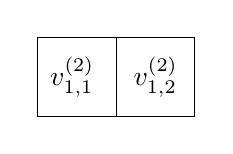
\begin{tikzpicture}[
  square/.style={
    draw,
    minimum width=1cm,
    minimum height=1cm,
    align=center
  }
]
\centering
\matrix[matrix of nodes,
        nodes={square},
        row sep=-\pgflinewidth,
        column sep=-\pgflinewidth] (grid) {
  $v_{1,1}^{(2)}$ &  $v_{1,2}^{(2)}$\\
};
\end{tikzpicture}

\[
v_{1,2}^{(1)} = \mat{0\\1\\0\\0}, \quad v_{1,1} = (C + 2\cdot I_4)v_{1,2} = \mat{-3&1&1&1\\-3&2&-1&-1\\0&0&3&0\\-6&1&1&4}\mat{0\\1\\0\\0} = \mat{1\\2\\0\\1}
\]

\[S = (v_{1,1}^{(1)}, v_{2,1}^{(1)}, v_{1,2}^{(2)}, v_{1,1}^{(2)}) = \mat{0&0&1&0\\1&1&2&1\\-1&0&0&0\\0&-1&1&0}\]

\paragraph{Die Inverse $S^{-1}$}
\begin{align*}
&\left(\begin{matrix}
0&0&1&0\\1&1&2&1\\-1&0&0&0\\0&-1&1&0
\end{matrix}
\;\;\middle|\;\;
\begin{matrix}
1&0&0&0\\0&1&0&0\\0&0&1&0\\0&0&0&1
\end{matrix}
\right)\rightsquigarrow
\left(\begin{matrix}
0&0&1&0\\1&0&3&1\\0&0&3&1\\0&1&0&0
\end{matrix}
\;\;\middle|\;\;
\begin{matrix}
1&0&0&0\\0&1&0&1\\0&1&1&1\\1&0&0&-1
\end{matrix}
\right)\\
\rightsquigarrow
&\left(\begin{matrix}
0&0&1&0\\1&0&0&0\\0&0&0&1\\0&1&0&0
\end{matrix}
\;\;\middle|\;\;
\begin{matrix}
1&0&0&0\\0&0&-1&0\\-3&1&1&1\\1&0&0&-1
\end{matrix}
\right)\\
S^{-1} =& \mat{0&0&-1&0\\1&0&0&-1\\1&0&0&0\\-3&1&1&1}
\end{align*}

\paragraph{Berechnung von $S^{-1}CS$}
\begin{align*}
J = S^{-1}CS &= \mat{0&0&-1&0\\1&0&0&-1\\1&0&0&0\\-3&1&1&1}\mat{-5&1&1&1\\-3&0&-1&-1\\0&0&1&0\\-6&1&1&2}\mat{0&0&1&0\\1&1&2&1\\-1&0&0&0\\0&-1&1&0}\\
&= \mat{0&0&-1&0\\0&0&0&-1\\-5&1&1&1\\6&-2&-2&-2}\mat{0&0&1&0\\1&1&2&1\\-1&0&0&0\\0&-1&1&0}\\
&= \mat{{\color{MediumVioletRed}1}&{\color{MediumVioletRed}0}&0&0\\{\color{MediumVioletRed}0}&{\color{MediumVioletRed}1}&0&0\\0&0&{\color{Green}-2}&{\color{Green}1}\\0&0&{\color{Green}0}&{\color{Green}-2}}
\end{align*}


\end{document}
